% Generated from first-principles-jul2026.ipynb -- do not hand-edit.
% Preamble: \usepackage{pgfplots} \pgfplotsset{compat=1.18}
\definecolor{upsetface}{HTML}{9AC1F2}
\definecolor{upsetedge}{HTML}{408AE6}
\definecolor{upsetshade}{HTML}{D2F1FA}
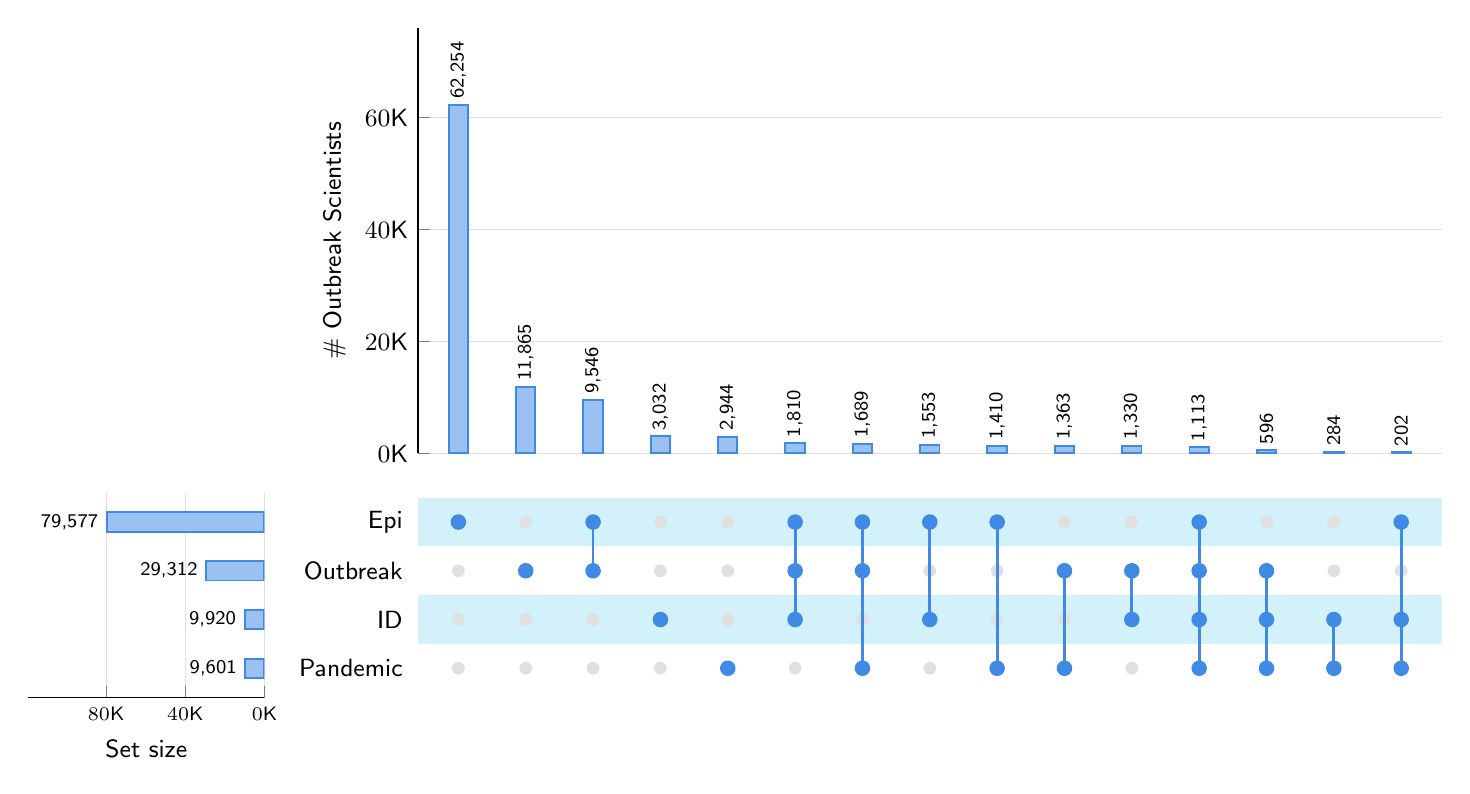
\begin{tikzpicture}[font=\sffamily\small]
%% ---- membership matrix (anchors the other two panels) -------------------
\begin{axis}[
  name=matrix, anchor=south west, at={(0cm,0cm)},
  width=13cm, height=2.6cm, scale only axis,
  % pgfplots defers ALL marks past ALL plot paths so they escape clipping, which paints the
  % grey dots over the connectors no matter the source order. This draws marks in order.
  clip marker paths=true,
  xmin=0.4, xmax=15.6, ymin=0.4, ymax=4.6,
  axis line style={draw=none}, tick style={draw=none},
  xtick=\empty, ytick={4,3,2,1},
  yticklabels={{Epi},{Outbreak},{ID},{Pandemic}},
  yticklabel style={anchor=east, xshift=-2pt},
]
  \fill[upsetshade] (axis cs:0.4,3.5) rectangle (axis cs:15.6,4.5);
  \fill[upsetshade] (axis cs:0.4,1.5) rectangle (axis cs:15.6,2.5);
  \addplot[only marks, mark=*, mark size=2.1pt, black!12] coordinates {(1,3) (1,2) (1,1) (2,4) (2,2) (2,1) (3,2) (3,1) (4,4) (4,3) (4,1) (5,4) (5,3) (5,2) (6,1) (7,2) (8,3) (8,1) (9,3) (9,2) (10,4) (10,2) (11,4) (11,1) (13,4) (14,4) (14,3) (15,3)};
  \addplot[upsetedge, line width=1pt, mark=none, forget plot] coordinates {(3,3) (3,4)};
  \addplot[upsetedge, line width=1pt, mark=none, forget plot] coordinates {(6,2) (6,4)};
  \addplot[upsetedge, line width=1pt, mark=none, forget plot] coordinates {(7,1) (7,4)};
  \addplot[upsetedge, line width=1pt, mark=none, forget plot] coordinates {(8,2) (8,4)};
  \addplot[upsetedge, line width=1pt, mark=none, forget plot] coordinates {(9,1) (9,4)};
  \addplot[upsetedge, line width=1pt, mark=none, forget plot] coordinates {(10,1) (10,3)};
  \addplot[upsetedge, line width=1pt, mark=none, forget plot] coordinates {(11,2) (11,3)};
  \addplot[upsetedge, line width=1pt, mark=none, forget plot] coordinates {(12,1) (12,4)};
  \addplot[upsetedge, line width=1pt, mark=none, forget plot] coordinates {(13,1) (13,3)};
  \addplot[upsetedge, line width=1pt, mark=none, forget plot] coordinates {(14,1) (14,2)};
  \addplot[upsetedge, line width=1pt, mark=none, forget plot] coordinates {(15,1) (15,4)};
  \addplot[only marks, mark=*, mark size=2.6pt, upsetedge] coordinates {(1,4) (2,3) (3,4) (3,3) (4,2) (5,1) (6,4) (6,3) (6,2) (7,4) (7,3) (7,1) (8,4) (8,2) (9,4) (9,1) (10,3) (10,1) (11,3) (11,2) (12,4) (12,3) (12,2) (12,1) (13,3) (13,2) (13,1) (14,2) (14,1) (15,4) (15,2) (15,1)};
\end{axis}

%% ---- intersection sizes -------------------------------------------------
\begin{axis}[
  name=bars, at={(matrix.north west)}, anchor=south west, yshift=0.5cm,
  width=13cm, height=5.4cm, scale only axis,
  ybar, bar width=7pt,
  xmin=0.4, xmax=15.6, ymin=0, ymax=75950,   % headroom for the rotated value label on the tallest bar
  axis x line=none, axis y line*=left,
  ylabel={\# Outbreak Scientists}, ylabel style={align=center},
  scaled y ticks=false, scaled y ticks={real:1000}, ytick scale label code/.code={}, yticklabel={\pgfmathprintnumber[precision=0]{\tick}K},
  ymajorgrids, grid style={black!12},
]
  \addplot[fill=upsetface, draw=upsetedge, line width=0.7pt] coordinates {(1,62254) (2,11865) (3,9546) (4,3032) (5,2944) (6,1810) (7,1689) (8,1553) (9,1410) (10,1363) (11,1330) (12,1113) (13,596) (14,284) (15,202)};
  \node[rotate=90, anchor=west, inner sep=2pt, font=\sffamily\scriptsize] at (axis cs:1,62254) {62,254};
  \node[rotate=90, anchor=west, inner sep=2pt, font=\sffamily\scriptsize] at (axis cs:2,11865) {11,865};
  \node[rotate=90, anchor=west, inner sep=2pt, font=\sffamily\scriptsize] at (axis cs:3,9546) {9,546};
  \node[rotate=90, anchor=west, inner sep=2pt, font=\sffamily\scriptsize] at (axis cs:4,3032) {3,032};
  \node[rotate=90, anchor=west, inner sep=2pt, font=\sffamily\scriptsize] at (axis cs:5,2944) {2,944};
  \node[rotate=90, anchor=west, inner sep=2pt, font=\sffamily\scriptsize] at (axis cs:6,1810) {1,810};
  \node[rotate=90, anchor=west, inner sep=2pt, font=\sffamily\scriptsize] at (axis cs:7,1689) {1,689};
  \node[rotate=90, anchor=west, inner sep=2pt, font=\sffamily\scriptsize] at (axis cs:8,1553) {1,553};
  \node[rotate=90, anchor=west, inner sep=2pt, font=\sffamily\scriptsize] at (axis cs:9,1410) {1,410};
  \node[rotate=90, anchor=west, inner sep=2pt, font=\sffamily\scriptsize] at (axis cs:10,1363) {1,363};
  \node[rotate=90, anchor=west, inner sep=2pt, font=\sffamily\scriptsize] at (axis cs:11,1330) {1,330};
  \node[rotate=90, anchor=west, inner sep=2pt, font=\sffamily\scriptsize] at (axis cs:12,1113) {1,113};
  \node[rotate=90, anchor=west, inner sep=2pt, font=\sffamily\scriptsize] at (axis cs:13,596) {596};
  \node[rotate=90, anchor=west, inner sep=2pt, font=\sffamily\scriptsize] at (axis cs:14,284) {284};
  \node[rotate=90, anchor=west, inner sep=2pt, font=\sffamily\scriptsize] at (axis cs:15,202) {202};
\end{axis}

%% ---- set sizes: TOTAL cardinality of each set, never a sum over the bars -
\begin{axis}[
  name=sizes, at={(matrix.south west)}, anchor=south east, xshift=-1.95cm,
  width=3.0cm, height=2.6cm, scale only axis,
  xbar, bar width=7pt, x dir=reverse,
  xmin=0, xmax=119366, ymin=0.4, ymax=4.6,
  ytick=\empty, axis y line=none, axis x line*=bottom,
  xlabel={Set size}, xtick={0,40000,80000},
  xmajorgrids, grid style={black!12},
  scaled x ticks={real:1000}, xtick scale label code/.code={},
  xticklabel={\pgfmathprintnumber[precision=0]{\tick}K},
  xticklabel style={font=\sffamily\scriptsize},
]
  \addplot[fill=upsetface, draw=upsetedge, line width=0.7pt] coordinates {(79577,4) (29312,3) (9920,2) (9601,1)};
  \node[anchor=east, inner sep=3pt, font=\sffamily\scriptsize] at (axis cs:79577,4) {79,577};
  \node[anchor=east, inner sep=3pt, font=\sffamily\scriptsize] at (axis cs:29312,3) {29,312};
  \node[anchor=east, inner sep=3pt, font=\sffamily\scriptsize] at (axis cs:9920,2) {9,920};
  \node[anchor=east, inner sep=3pt, font=\sffamily\scriptsize] at (axis cs:9601,1) {9,601};
\end{axis}
\end{tikzpicture}